%%%%%%%%%%%%%%%%%%%%%%%%%%%%%%%%
% Tables
%%%%%%%%%%%%%%%%%%%%%%%%%%%%%%%%

\clearpage
\section{Tables}

\begin{table}[!h]
\caption{Countries and data}
\resizebox{\textwidth}{!}{
\begin{tabular}{llll}
\toprule
Countries       & Datasets & Years & Survey period \\ \midrule
1) Australia       & Household, Income and Labour Dynamics in Australia  \citep{hilda_household_2022}   & 2001 -   & Annual \\
2) Germany         & Socioeconomic Panel \citep{soep_2020}   & 1984 - & Annual \\
3) Italy           & Survey on Household Income and Wealth \citep{shiw_historical_2019}   & 1977 (2000) - & Biannual \\
4) Japan  \citeyearpar{jhpskhps_keio_2019}           & a) Keio Household Panel Survey (KHSP) & 2004 -  & Annual  \\
                    & b) Japan Household Panel Survey (JHPS) & 2009 -  & Annual \\
5) Korea           & Korean Labour \& Income Panel Study \citep{klips_korean_2020}   & 1998 - & Annual  \\
6) Netherlands      & a) Labour Supply Panel \citep{lsp_arbeidsaanbodpanel_2016} & 1984 - 2014 & Biannnual  \\
                        & b) Longitudinal Internet studies for the Social Sciences \citep{liss_longitudinal_2020} & 2008 - & Annual \\
7) Switzerland     & Swiss Household Panel \citep{shp_swiss_2020}  &  1999 - & Annual    \\
8) United Kingdom  \citeyearpar{bhpsukhls_university_2022}  & a) British Household Panel Study (BHPS) & 1991 - 2008 & Annual \\
  & b) United Kingdom Household Longitudinal Study (UKHLS) & 2009 -  & Annual \\
\bottomrule
\end{tabular}}
\\ 
\scriptsize{Notes: In Italy, panel data from the SHIW are available since 1977, but the variable for temporary employment is only available after the year 2000.  In Japan and the United Kingdom, the two data sets are harmonized prior to release by the agency responsible for making the data available to researchers.  In the Netherlands, the LSP represents the main source of data, but we use the LISS as a sensitivity check.  For more details on each data set, please see Appendix \ref{appendix:data}}
\label{table_country_data}
\end{table}

\begin{table}[!h]
    \caption{Sample filter steps}
    \resizebox{\textwidth}{!}{\begin{tabular}{llll}
   \toprule 
 
&  & 
\multicolumn{2}{l}{Total (all countries)}
\\  
 
 
\multicolumn{1}{l}{Step} & 
\multicolumn{1}{l}{Description} 
& n & $\Delta$
\\ 
\cmidrule(lr){1-2}
\cmidrule(lr){3-4}
\\[-1.8ex]  
 
0 & Raw data & 415,771 &  \\ 
  1 & Panel years between 2000 and 2018 & 367,032 & -12\% \\ 
  2 & Prime age (25 - 54) & 210,900 & -43\% \\ 
  3 & Labour force participant (employed or unemployed) & 181,607 & -14\% \\ 
  4 & Unemployed or employed with contract type & 165,347 & -9\% \\ 
  5 & Unemployed or employed with wages & 164,001 & -1\% \\ 
  6 & Unemployed or employed with monthly hours between 40 and 320 & 158,534 & -3\% \\ 
  7 & Non missing education or gender & 156,683 & -1\% \\ 
  8 & Hourly wages within the top/bottom 0.005 percentile & 155,151 & -1\% \\ 
  9 & Sample A: At least 3 observations & 79,466 & -49\% \\ 
  10 & Sample B: + always employed & 73,501 & -8\% \\ 
   \bottomrule\end{tabular}
}
    \label{table_sample_filter_steps_country}
    \scriptsize{Notes: n refers to unique individuals. $\Delta$ refers to percent change from previous step.  Please see Appendix \ref{appendix:sample_selection} for more details on the sample selection criteria, including country specific frequency counts.}
\end{table}


%%%%%%%%%%%%%%%%%%%%%%%%%%%%%%%%
% Graphs
%%%%%%%%%%%%%%%%%%%%%%%%%%%%%%%%
\clearpage
\section{Graphs}

\begin{sidewaysfigure}[h!]
    \caption{Estimated wage effect of temporary employment and transitions into and out of temporary employment}
    \resizebox{\textwidth}{!}{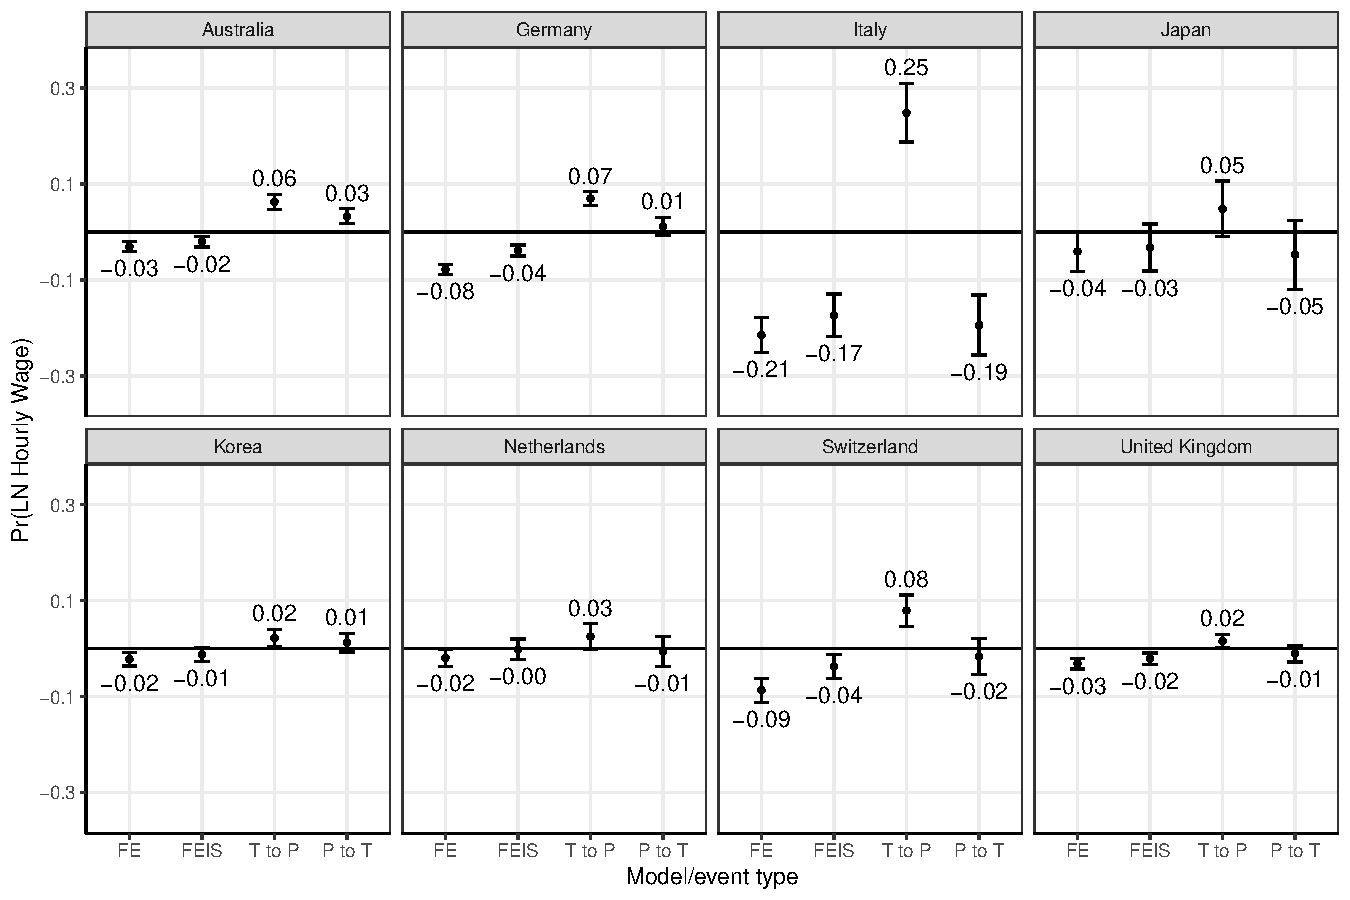
\includegraphics{../../../graphs/graph_multiple_events_contyp_paper.pdf}}
    \label{graph_contyp}
    \footnotesize{Note: Authors calculations using sample B in country-specific panel data, where all individuals are employed in either a temporary or permanent contract.  Within each country cell, the graph displays four parameter estimates from three models: FE, FEIS, and AFE (T $\rightarrow$ P and P $\rightarrow$ T).  The interpretation is that the negative coefficients identified in the FE model and partially explained by the FEIS model do not indicate that the wage effects of temporary employment are negative.  Instead, the negative effects are better understood as the result of two transitions, neither of which are negative (except in Italy), even if one is more positive than the other.  Raw coefficients and standard errors are shown in Appendix \ref{appendix:coefficients}.}
\end{sidewaysfigure}

\begin{sidewaysfigure}
    \caption{Estimated wage effect over time of transitions between contract types}
    \resizebox{\textwidth}{!}{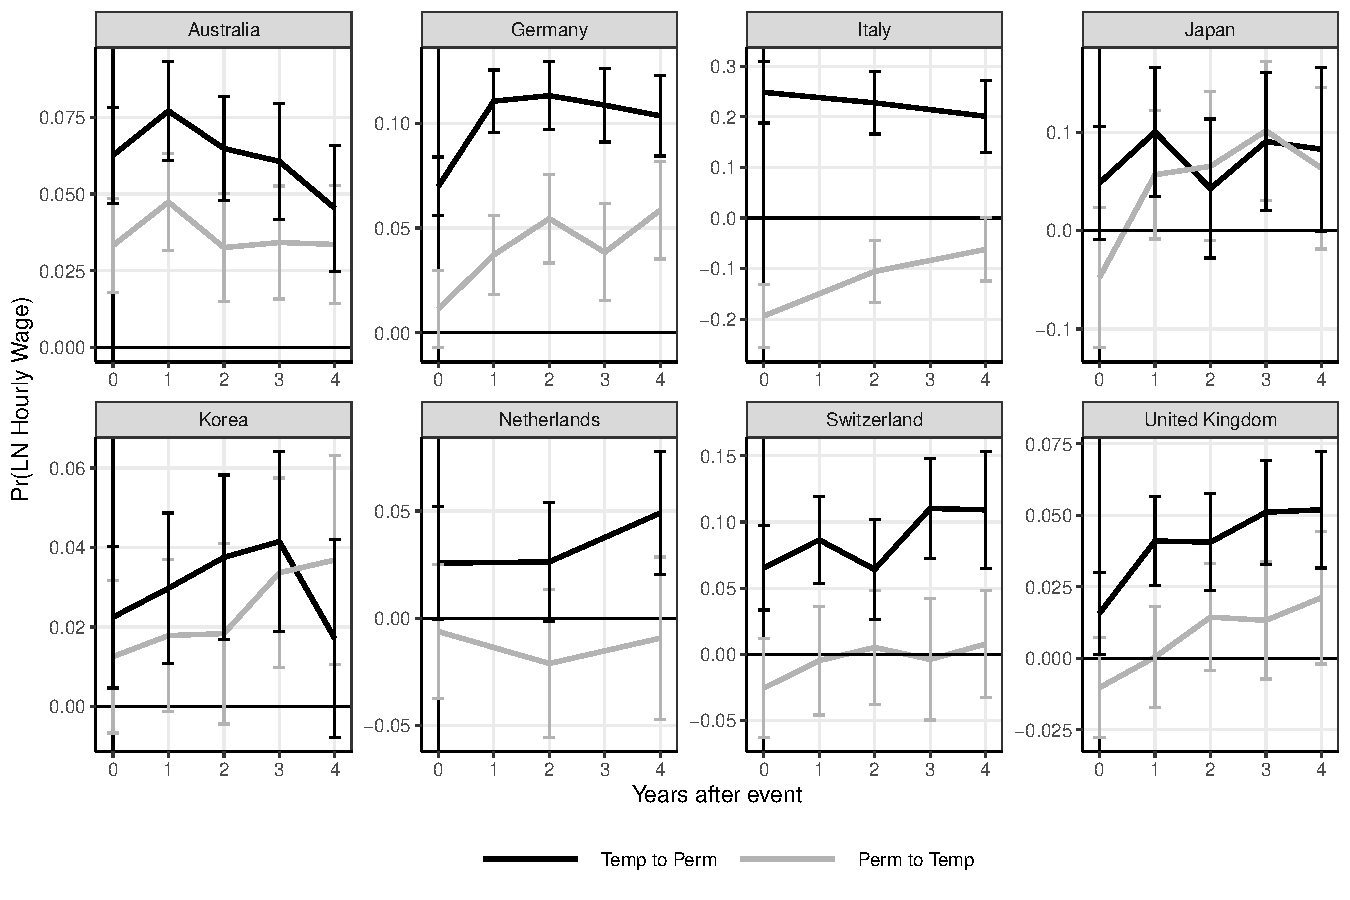
\includegraphics{../../../graphs/graph_multiple_events_contyp_post_paper.pdf}}
    \label{graph_contyp_post}
    \footnotesize{Note: Authors calculations using sample B in country-specific panel data, where all individuals are employed in either a temporary or permanent contract.  Within each country cell, the graph displays estimates from the asymmetric fixed effects (AFE) model \ref{eq:model_afe_temp} on the the year of a given transition (0) as well as up to four years afterward for transitions from temporary to permanent (Temp to Perm) and permanent to temporary (Perm to Temp).  The main interpretation is that transitions from permanent into temporary contracts remain less positive over time than transition from temporary into permanent contracts, but not negative (except Italy).}
\end{sidewaysfigure}

\begin{sidewaysfigure}
    \caption{Estimated effect of transitions out of unemployment by contract type on wages at point in time}
    \resizebox{\textwidth}{!}{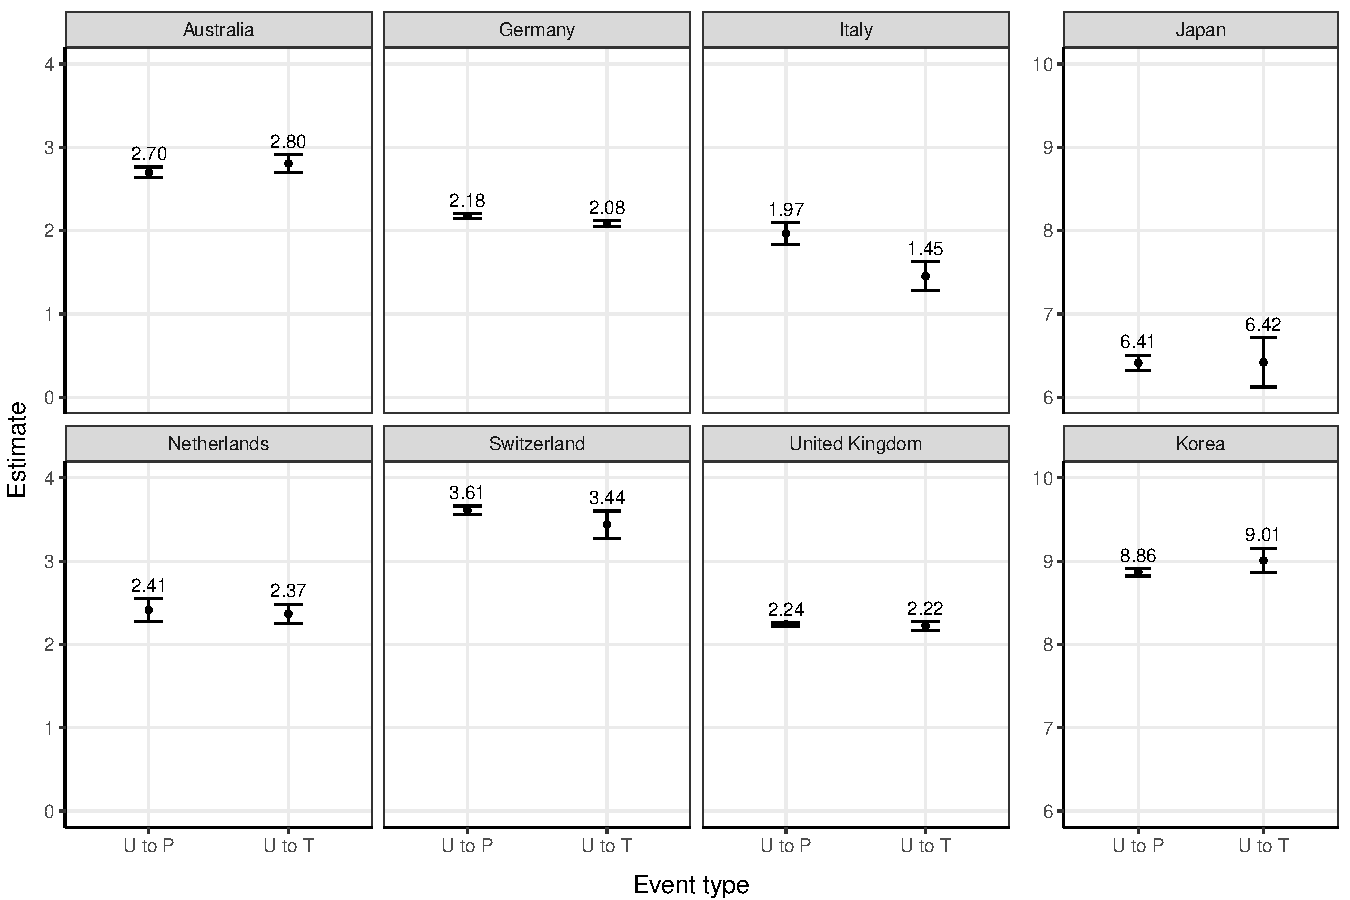
\includegraphics{../../../graphs/graph_multiple_events_unmp_better_paper.pdf}}
    \label{graph_unmp}
    \footnotesize{Note: Authors calculations using sample A in country-specific panel data, where all individuals are employed in either a temporary or permanent contract.  Within each country cell, the graph displays two parameter estimates from the asymmetric fixed effects (AFE) model \ref{eq:model_afe_unmp}: transitions from unemployment to permanent (U to P) and unemployment to temporary (U to T).  The main interpretation is that, with the exception of Italy and Germany (to a lesser degree), there is little difference in the wage effects of transitions out of unemployment into permanent or temporary contracts.}
\end{sidewaysfigure}

\begin{sidewaysfigure}
    \caption{Estimated effect of transitions out of unemployment by contract type on wages over time}
    \resizebox{\textwidth}{!}{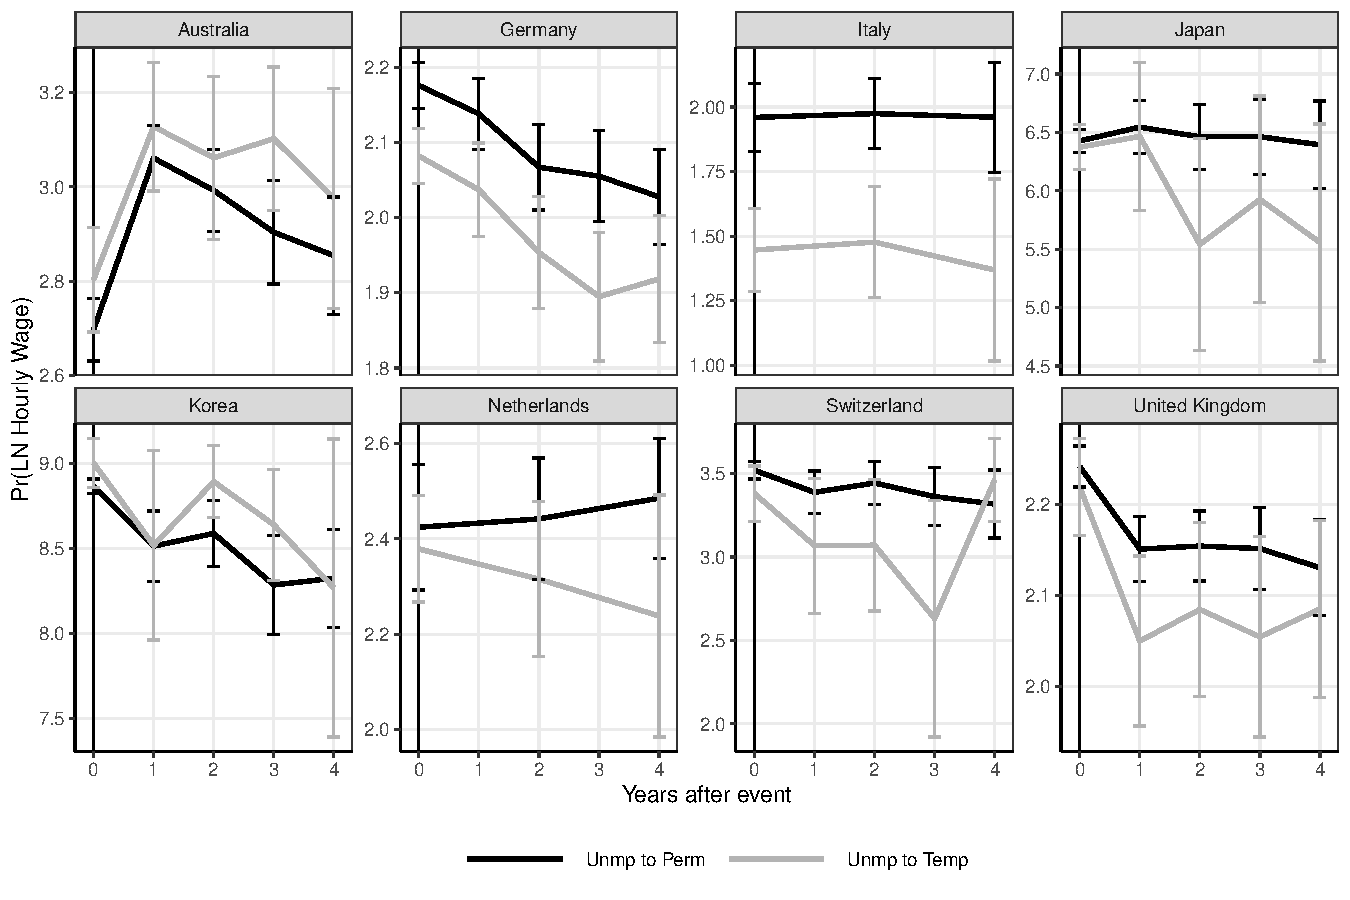
\includegraphics{../../../graphs/graph_multiple_events_unmp_post_free_scale.pdf}}
    \label{graph_unmp_post}
    \footnotesize{Note: Authors calculations using sample A in country-specific panel data, where all individuals are employed in either a temporary or permanent contract.  The graph displays parameter estimates in the periods including and after transitions from temporary to permanent (Unmp to Perm) and permanent to temporary (Unmp to Temp) from the asymmetric fixed effects (AFE) model \ref{eq:model_afe_unmp}.  With the exception of Italy and Germany, differences in wage effects over time following transitions out of unemployment between remain insignificant.}
\end{sidewaysfigure}
